%&inleiding
%% !TeX program = pdflatex
\documentclass[../presentatie.tex]{subfiles}

\begin{document}
    %\section{Inleiding}

    %\begin{frame}
    %	\begin{tabular}{p{0.5\textwidth}p{0.5\textwidth}}
    %		%\dimexpr 0.5\textheight-\height\relax
    %		\adjustbox{padding={0pt {\dimexpr (0.5\textheight-\height)/2\relax} {0pt} {\dimexpr (0.5\textheight-\height)/2\relax}},bgcolor=blue!5!white}{
    %			Websites
    %		} & \adjustbox{}{
    %			Apps
    %		}\\
    %		\adjustbox{}{
    %			Wikipedia
    %		} & \adjustbox{}{
    %			\LaTeX
    %		}
    %	\end{tabular}
    %\end{frame}
    \clearrecentlist
    
    \begin{frame}
    	\frametitle{\LaTeX{} vs Word}
    	
    	\begin{columns}
    		\begin{column}{0.5\textwidth}
    			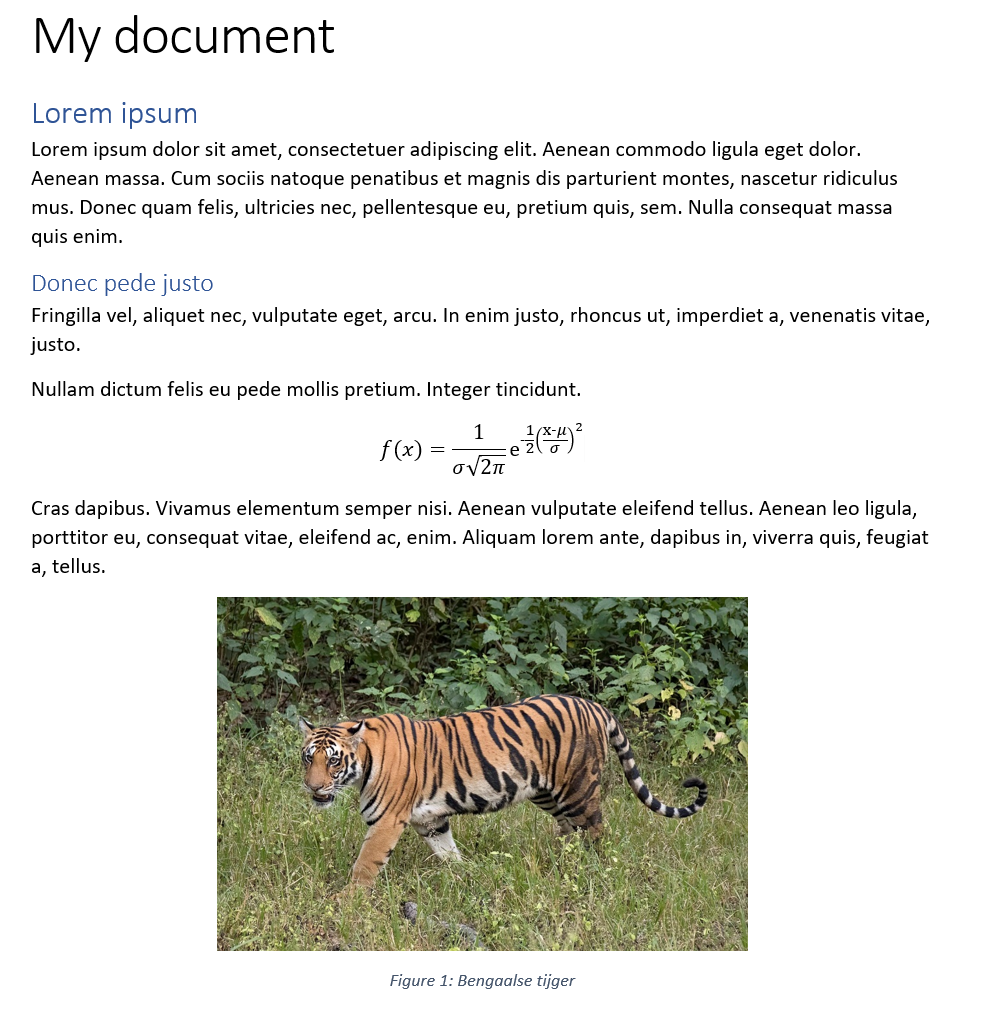
\includegraphics[width=\linewidth,height=0.8\textheight,keepaspectratio]{assets/basicDocWordSnippet.png}
    		\end{column}
	    	\begin{column}{0.5\textwidth}
    			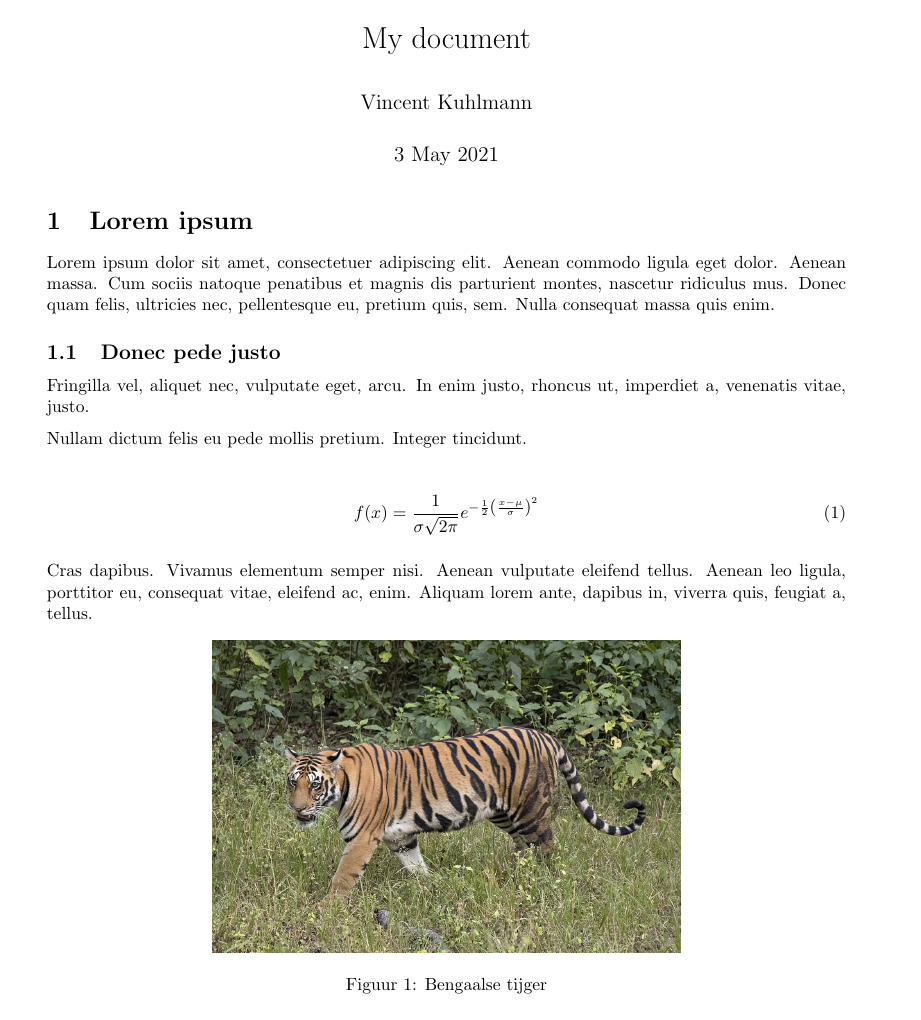
\includegraphics[width=\linewidth,height=0.8\textheight,keepaspectratio]{assets/basicDocLaTeXSnippet.png}
	    	\end{column}
    	\end{columns}
    \end{frame}

	\begin{frame}
		\frametitle{\LaTeX{} vs Word}
		
		\bgroup
		\setlength{\fboxsep}{0pt}
		\fbox{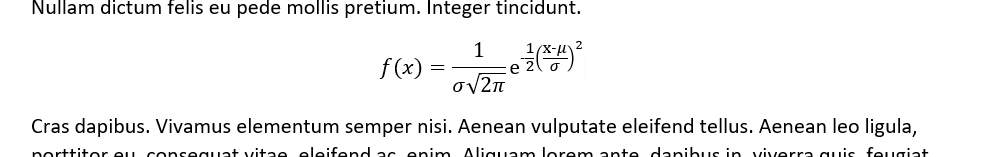
\includegraphics[width=\linewidth,height=0.5\textheight,keepaspectratio]{assets/basicDocWordSnippetEq.png}}
		\medskip
		
		\fbox{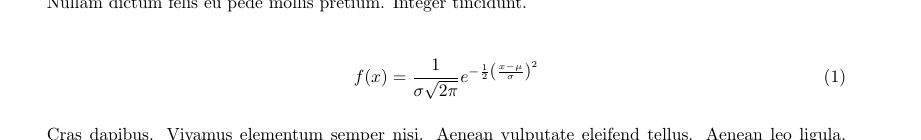
\includegraphics[width=\linewidth,height=0.5\textheight,keepaspectratio]{assets/basicDocLaTeXSnippetEq.png}}
		\egroup
	\end{frame}

%    \begin{frame}
%	\frametitle{\LaTeX{} vs Word}
%	
%	\begin{columns}
%			\begin{column}{0.5\textwidth}
%				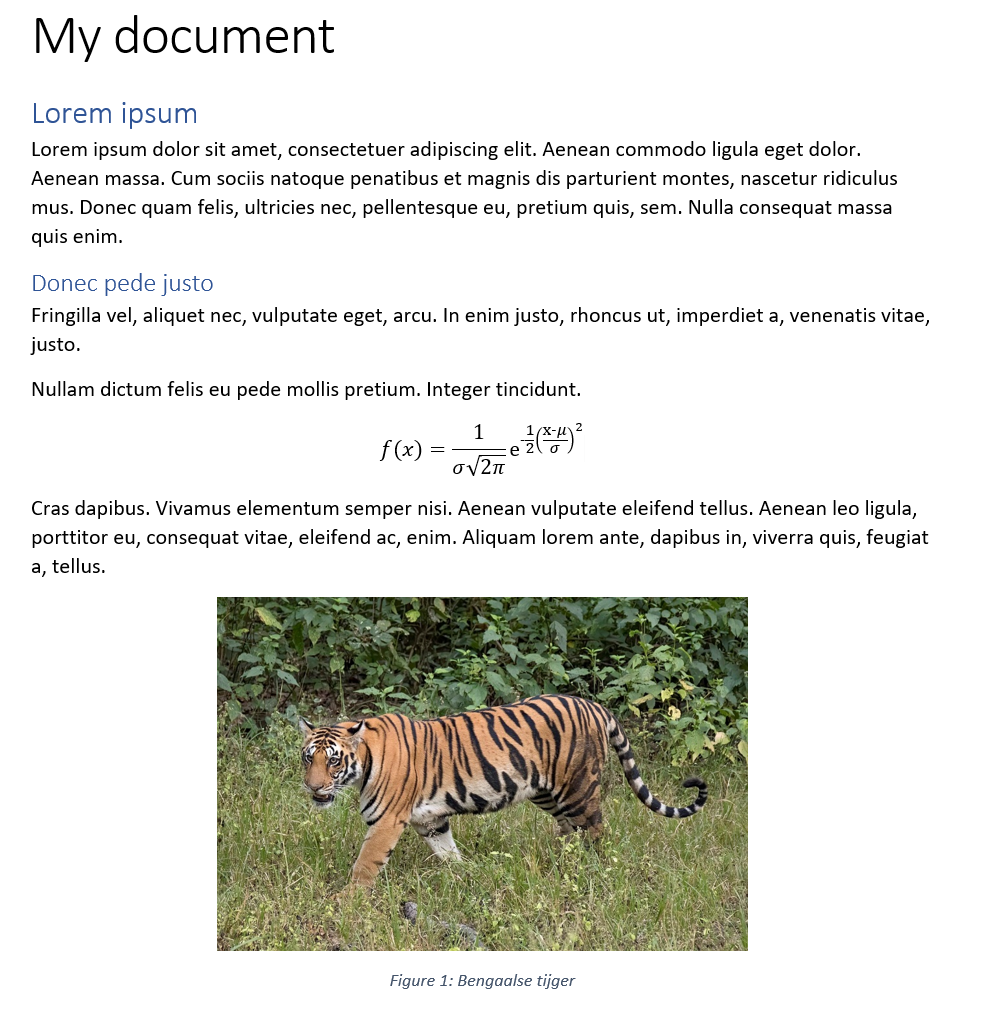
\includegraphics[width=\linewidth,height=0.8\textheight,keepaspectratio]{assets/basicDocWordSnippet.png}
%			\end{column}
%			\begin{column}{0.5\textwidth}
%				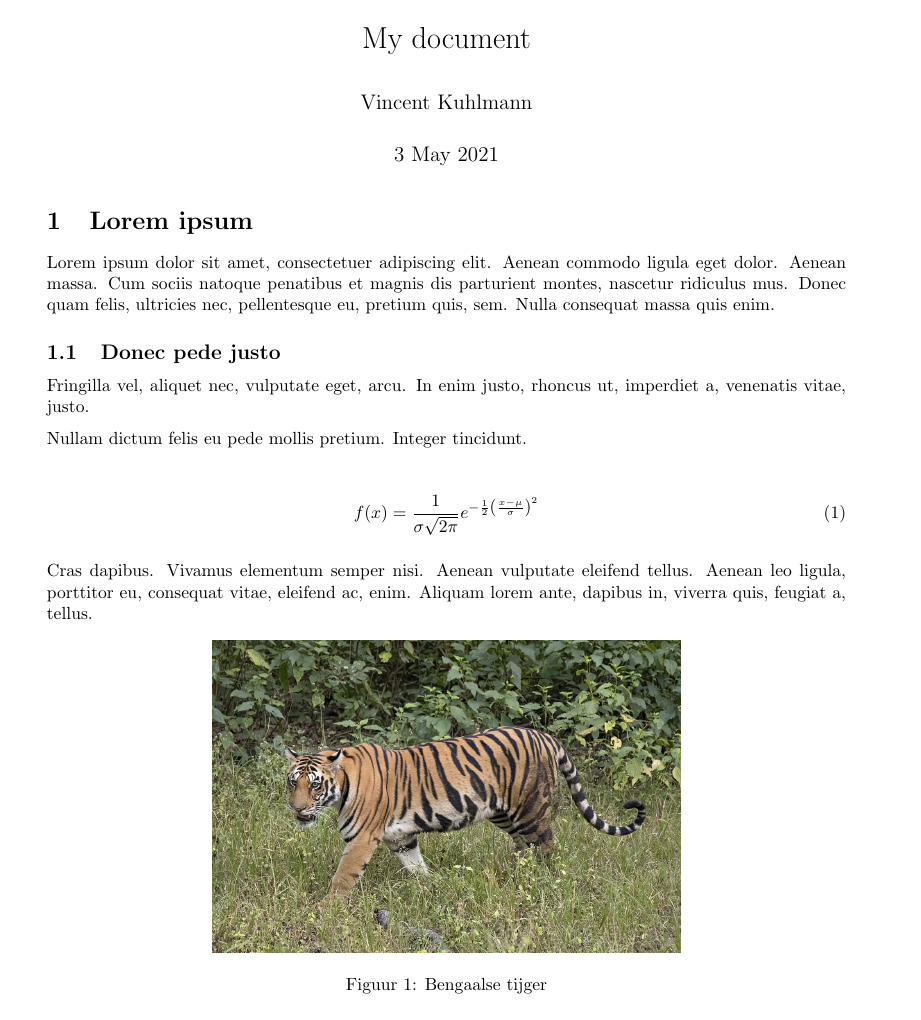
\includegraphics[width=\linewidth,height=0.8\textheight,keepaspectratio]{assets/basicDocLaTeXSnippet.png}
%			\end{column}
%		\end{columns}
%	\end{frame}

    
    \begin{frame}
        \frametitle{\LaTeX{} vs Word}

        \only<-1>{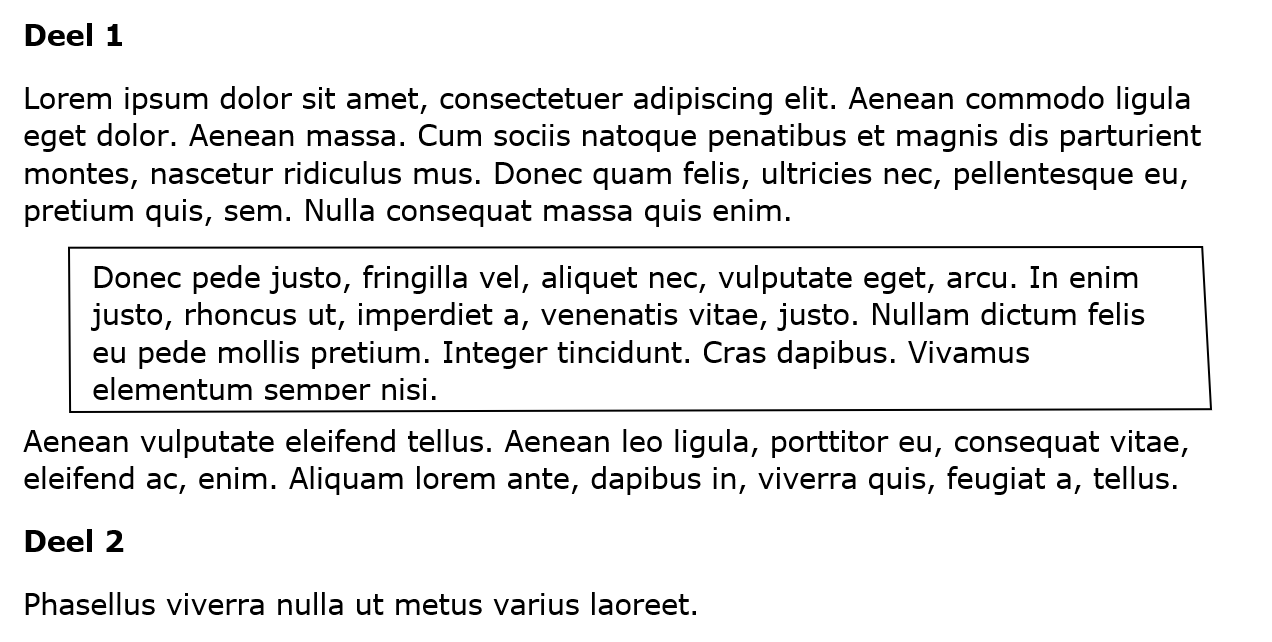
\includegraphics[width=\linewidth,height=0.8\textheight,keepaspectratio]{assets/wordkader2.png}}
        \unless\ifishandout
        \only<2->{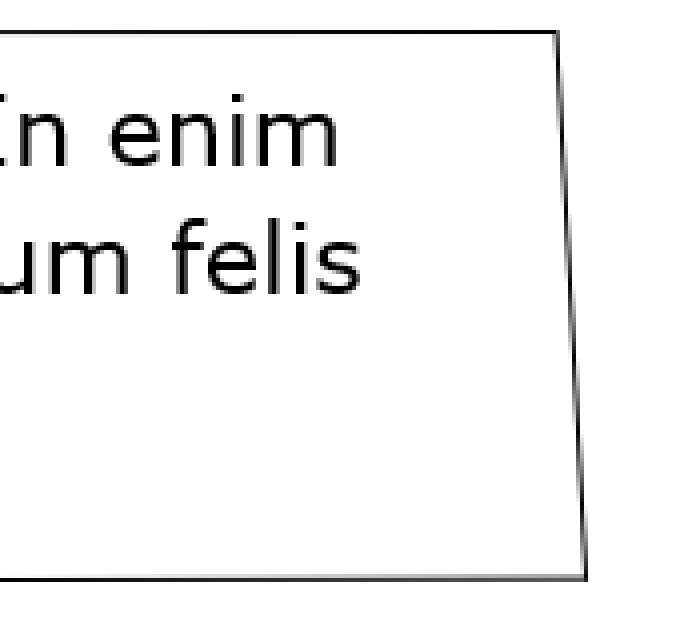
\includegraphics[width=\linewidth,height=0.8\textheight,keepaspectratio]{assets/wordkaderRand.png}}
        \fi

    \end{frame}

	\begin{saveblock}{basicDocCode}
		\begin{highlightblock}[linewidth=\textwidth,gobble=12]
			\title{My document}
			\author{Vincent Kuhlmann}
			\date{3 May 2021}
			
			\begin{document}
			\maketitle		
			\section{Lorem ipsum}
			Lorem ipsum dolor sit amet, consectetuer ...

			\begin{align}
				f(x) = \dfrac{1}{\sigma\sqrt{2\pi}} e^{
					-\frac{1}{2}\left(\frac{x-\mu}{\sigma}\right)^2}
			\end{align}
		\end{highlightblock}
	\end{saveblock}

	\addtorecentlist{tekst}

	\begin{frame}
		\frametitle{\LaTeX{} vs Word}
		
		Andere aanpak: Tekst!
		\pause
		\bigskip
		\useblock{basicDocCode}
	\end{frame}

    \addtorecentlist{veel}

    \begin{frame}
        \frametitle{Websites \& Apps: Tekst vs Visueel}
        \begin{columns}
            \begin{column}{0.6\textwidth}
                \vspace{10px}
                %\adjustbox{set height=4cm,left=\textwidth,bgcolor=gray,margin=10pt}{}
                \unless\ifishandout
                    \only<-1>{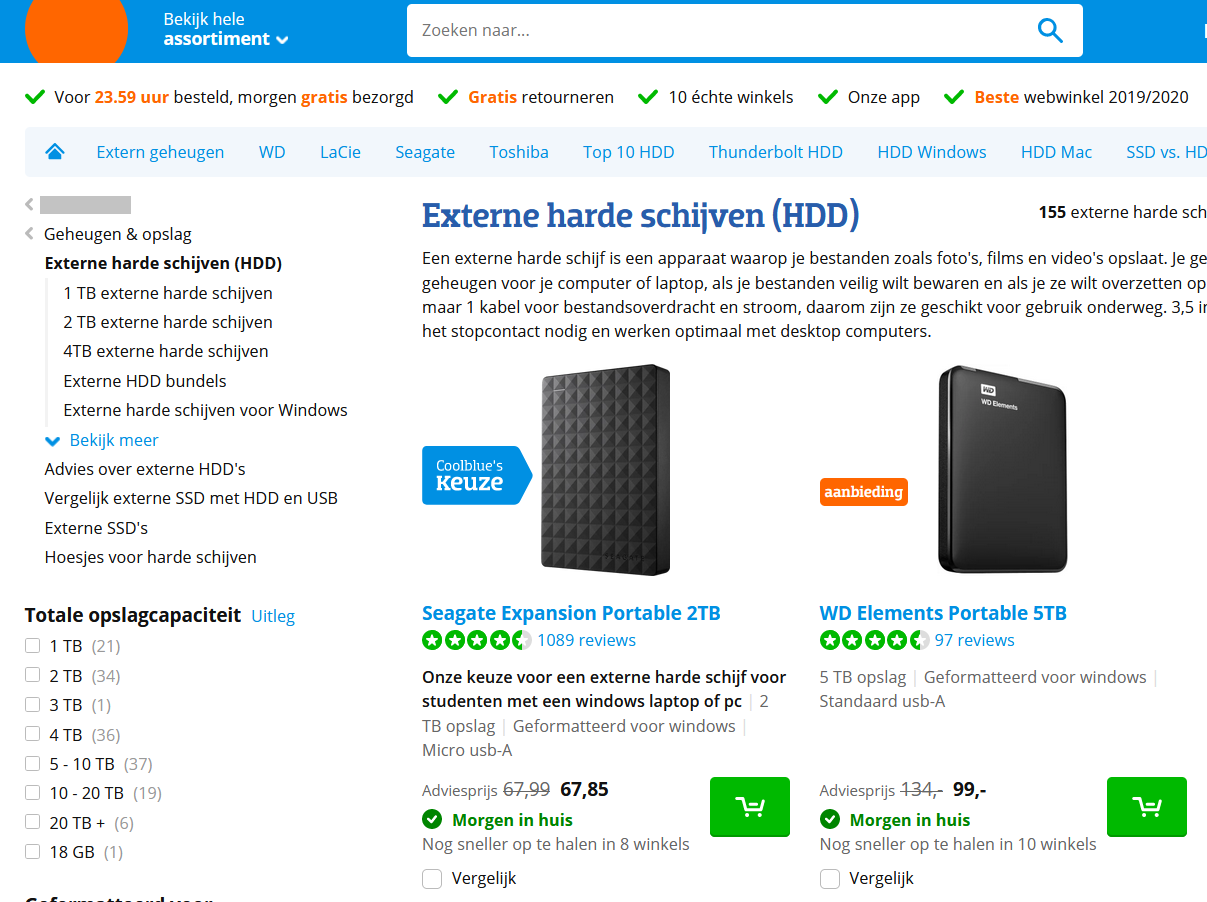
\includegraphics[width=\linewidth]{assets/websiteVisual.png}}
                \fi
                \only<2->{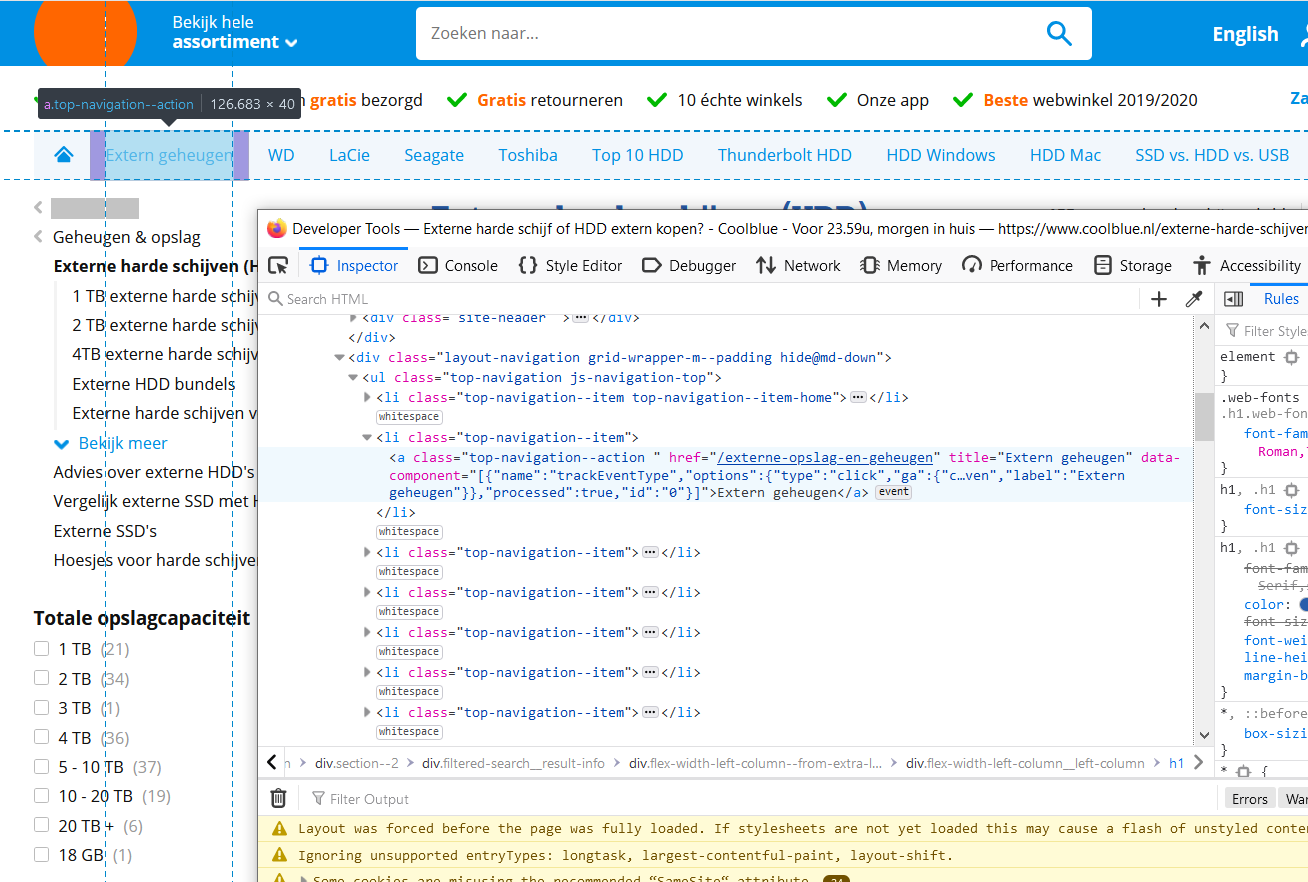
\includegraphics[width=\linewidth]{assets/websiteSource.png}}
            \end{column}
            \begin{column}{0.45\textwidth}
                \only<3->{\setul{1.5pt}{1pt}\setulcolor{red}\ul{Tekst = Veel informatie}}
                \begin{itemize}
                    \item Aanpassen aan schermgroottes
                    \item Interactiviteit
                    \item Dynamische inhoud
                    \item Herhalende elementen
                \end{itemize}
            \end{column}
        \end{columns}
    \end{frame}

    \begin{frame}
        \frametitle{Wikipedia: Tekst vs Visueel}
        \begin{columns}
            \begin{column}{0.4\textwidth}
                %\adjustbox{set height=4cm,left=\textwidth,bgcolor=gray,margin=10pt}{}
                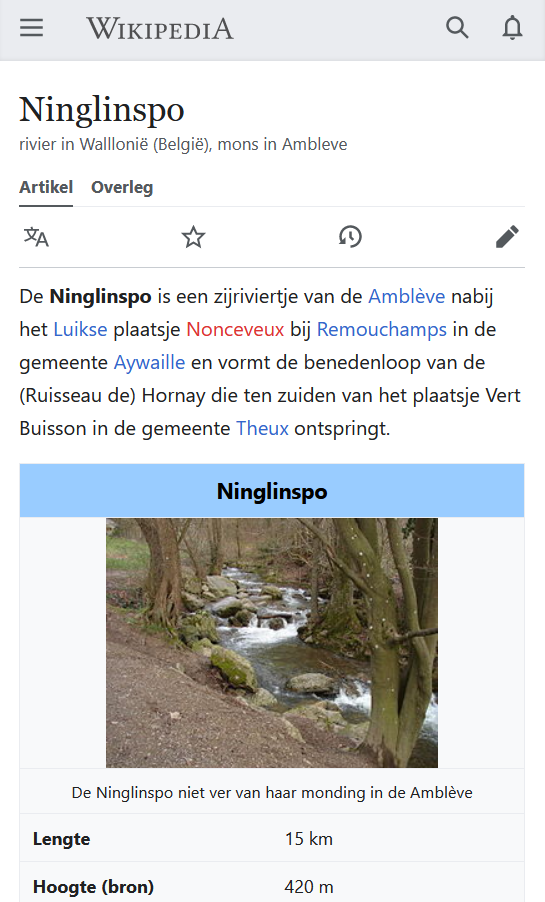
\includegraphics[width=\linewidth,height=0.85\textheight,keepaspectratio]{assets/wikipediaVisual}
            \end{column}
            \begin{column}{0.6\textwidth}
                
                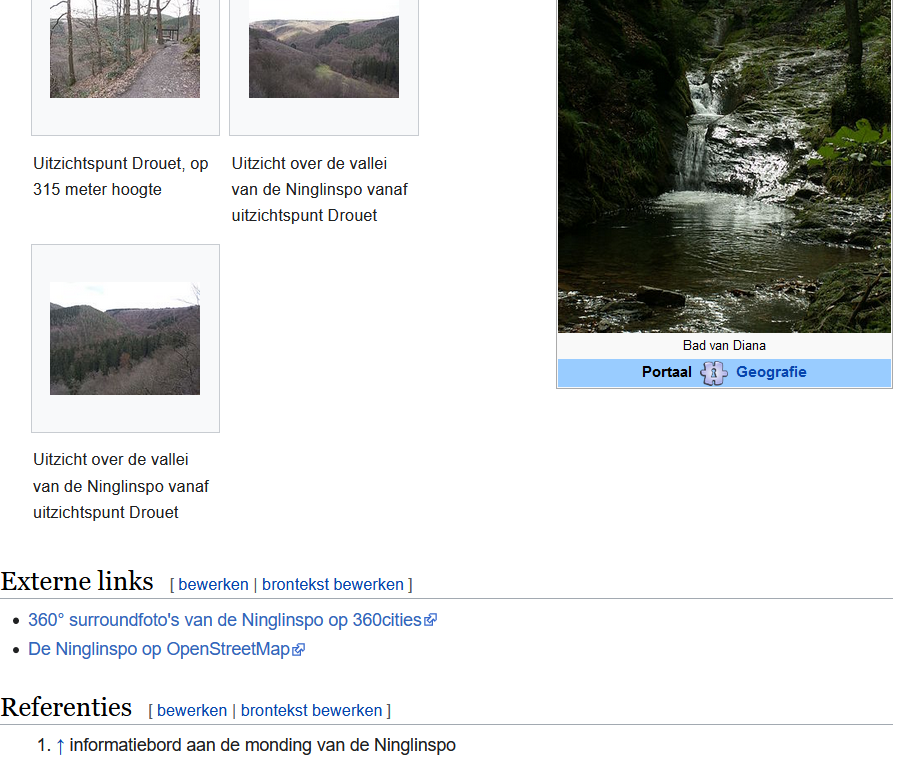
\includegraphics[width=\linewidth,height=0.85\textheight,keepaspectratio]{assets/wikipediaVisual3}
                %
    %			{\setul{1.5pt}{1pt}\setulcolor{red}\ul{Tekst = Informatie}}
    %			\begin{itemize}
    %				\item Focus op betekenis
    %				\item Stijl komt achteraf \textrightarrow{} Consistent en flexibel
    %			\end{itemize}
            \end{column}
        \end{columns}
    \end{frame}

    \begin{saveblock}{ninglinspoSource1}
        \begin{Verbatim}[tabsize=4,gobble=8]
        {{Infobox rivier
                | naam          = Ninglinspo
                | afbeelding    = Ninglinspo - arrivée du cours d'eau à Sedoz.jpg
                | onderschrift  = De Ninglinspo niet ver van haar monding in de Amblève
                | lengte        = 15
                | hoogte        = 420
                | hoogtemonding = 270
                | verhang       = 
                | debiet        = 
                | oppervlakte   = 5m^3
                | oorsprong     = Vert-Buisson ([[Theux]])
                | uitmonding    = [[Amblève (rivier)|Amblève]]
                | stroomgebied  = [[stroomgebied van de Maas|Maas]]
                | stroomtdoor   = [[Luik (provincie)|Luik]]
                | zijrivieren   = 
                | plaatsen      = 
                | bevaarbaar    = 
                | afbeelding2   = Ninglinspo,_Nonceveux,_ruisseau_de_Belgique,_cascade,_vallée_Amblève.jpg
                | onderschrift2 = Bad van Diana
                | afbeelding3   = 
                | onderschrift3 = 
        }}

        De '''Ninglinspo''' is een zijriviertje van de [[Amblève (rivier)|Amblève]] nabij het [[Luik
        (provincie)|Luikse]] plaatsje [[Nonceveux]] bij [[Remouchamps]] in de gemeente [[Aywaille]]
        en vormt de benedenloop van de (Ruisseau de) Hornay die ten zuiden van het plaatsje Vert
        Buisson in de gemeente [[Theux]] ontspringt.
        
        De rivier dankt haar vreemde naam aan een fout door de Franse cartografen in 1876. Ze
        verwarden de naam van de rivier met die van een veld waar de rivier in de Amblève stroomt.
        De oorspronkelijke naam is eigenlijk de "Doulneux" welke aangeeft dat het afkomstig is van
        een Els. Er werd reeds gesproken over de rivier in 647 met de oorspronkelijke naam in het
        charter van [[Sigibert III]]. <ref>informatiebord aan de monding van de Ninglinspo</ref>
        \end{Verbatim}
    \end{saveblock}
    \begin{saveblock}{ninglinspoSource2}
        \begin{Verbatim}[tabsize=4,gobble=8]
        De Ninglinspo is de enige [[Bergrivier (geologie)|bergrivier]] van België. Zij stroomt door
        een gebied dat sinds 1949 beschermd gebied is. De loop van de Ninglinspo daalt van 420 meter
        naar 170 meter, is 3 kilometer lang en heeft hierdoor een gemiddeld verval van
        8%. Ze overbrugt een hoogteverschil van 250 meter. De grootste waterval in de rivier is de
        [[Waterval van de Chaudière]], ze mondt uit in de Amblève net nadat deze in de Fonds de
        Quarreux overgaat. Door de erosie van het snelle en wervelende water ontstonden er enkele
        diepe, nauwe uithollingen die de bassins onderling verbinden. Deze bassins kregen poëtische
        namen zoals "bad van het hert", "Bad van Diana", "Bubbels van de ketel", "Bad van de
        waternimfen", "Bad van Venus",...
        
        <gallery>
        Bestand:Ninglinspo-Point de vue Drouet (3).jpg|Uitzichtspunt Drouet, op 315 meter hoogte
        Bestand:Ninglinspo-Point de vue Drouet (2).jpg|Uitzicht over de vallei van de Ninglinspo 
        vanaf uitzichtspunt Drouet
        Bestand:Ninglinspo-Point de vue Drouet (1).jpg|Uitzicht over de vallei van de Ninglinspo 
        vanaf uitzichtspunt Drouet
        </gallery>
        
        == Externe links ==
        * [http://www.360cities.net/search/ninglinspo 360° surroundfoto's van de Ninglinspo op 
        360cities]
        * [https://www.openstreetmap.org/way/581386904#map=15/50.4621/5.7590&layers=N De Ninglinspo
        op OpenStreetMap]
        
        == Referenties ==
        {{References}}
        
        {{Commonscat}}
        {{Coor title dms|50|28|7.51|N|5|44|48.82|E|scale:12500_type:river_region:BE}}
        
        [[Categorie:Rivier in Luik (provincie)]]
        [[Categorie:Aywaille]]
        [[Categorie:Beschermd erfgoed in Wallonië]]
        \end{Verbatim}
    \end{saveblock}
    
    \begin{frame}
    %	\adjustbox{max height=0.9\textheight,max width=0.9\textwidth}{
    %		\useblock{ninglinspoSource1}
    %	}
        \begin{columns}
            \begin{column}{0.6\textwidth}
                \adjustbox{max height=0.9\textheight,max width=0.6\textwidth}{
                    \useblock{ninglinspoSource1}
                }
            \end{column}
            \begin{column}{0.6\textwidth}
                \adjustbox{max height=0.9\textheight,max width=0.6\textwidth}{
                    \useblock{ninglinspoSource2}
                }
            \end{column}
        \end{columns}
    \end{frame}

    \addtorecentlist{minimalistisch}
    
    \begin{frame}
        \frametitle{Wikipedia: Tekst vs Visueel}
        \begin{columns}
            \begin{column}{0.6\textwidth}
                \centering
                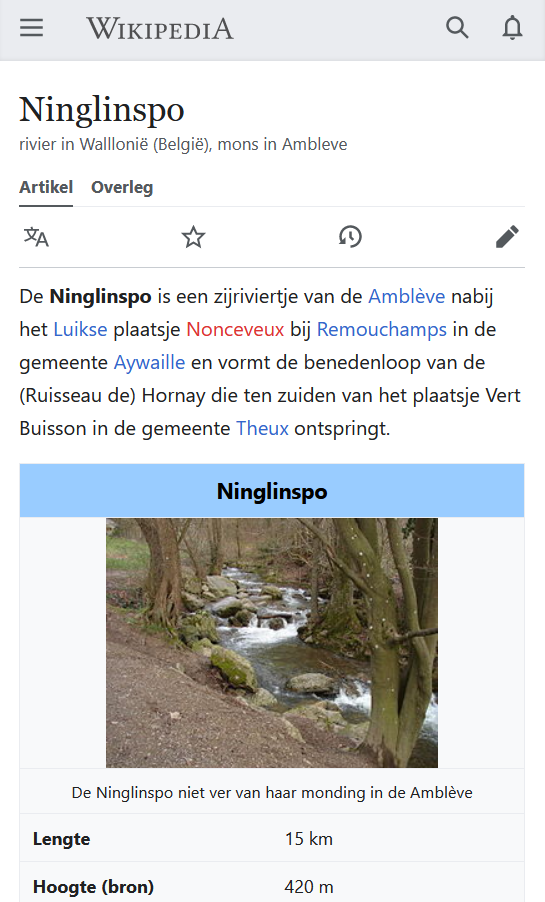
\includegraphics[width=\linewidth,height=0.7\textheight,keepaspectratio]{assets/wikipediaVisual}
            \end{column}
            \begin{column}{0.45\textwidth}
                \only<2->{\setul{1.5pt}{1pt}\setulcolor{red}\ul{Tekst = Minimalistische informatie}}
                \begin{itemize}
                    \item Focus op betekenis
                    \item Stijl komt achteraf \textrightarrow{} Consistent en flexibel
                \end{itemize}
            \end{column}
        \end{columns}
    \end{frame}

    \addtorecentlist{simpel}
    
    \begin{frame}
        \frametitle{WhatsApp: Tekst vs Visueel}
        \begin{columns}
            \begin{column}{0.5\textwidth}
                %\adjustbox{set height=4cm,left=\textwidth,bgcolor=gray,margin=10pt}{}
                
\includegraphics[width=\linewidth]{assets/whatsappStyles2.png}
                
                \bigskip
                
                %
\includegraphics[width=\linewidth]{whatsappStylesResultCropped.jpg}
                
\includegraphics[width=\linewidth]{assets/whatsappStylesResult2.png}
            \end{column}
            \begin{column}{0.5\textwidth}
                \only<2->{\setul{1.5pt}{1pt}\setulcolor{red}\ul{Tekst = Simpele informatie}}
                \begin{itemize}
                    \item Inzichtelijk
                    \item Beperk aantal knoppen op het scherm
                    \item Eenvoud voor programmeur
                \end{itemize}
            \end{column}
        \end{columns}
    \end{frame}
    
    \begin{frame}
        \begin{columns}
            \begin{column}{0.5\textwidth}\centering
                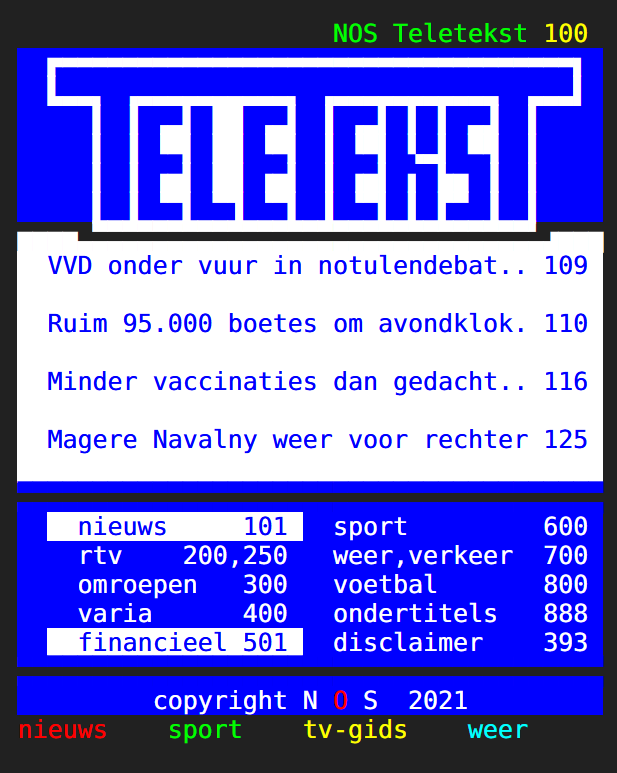
\includegraphics[width=\linewidth,height=0.9\textheight,keepaspectratio]{assets/teletekst.png}
            \end{column}
            \begin{column}{0.5\textwidth}\centering
                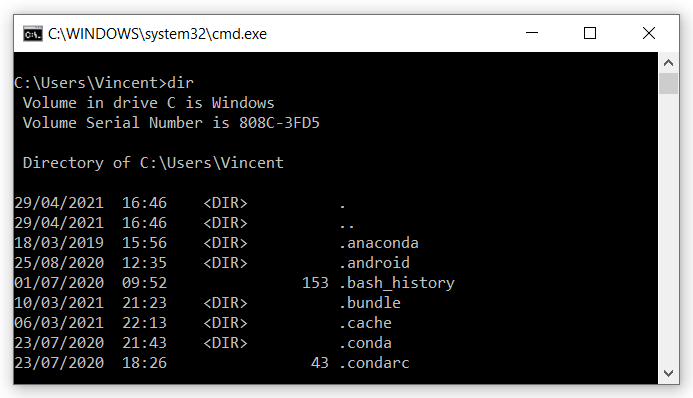
\includegraphics[width=\linewidth]{assets/commandPrompt.png}
                
                \medskip
                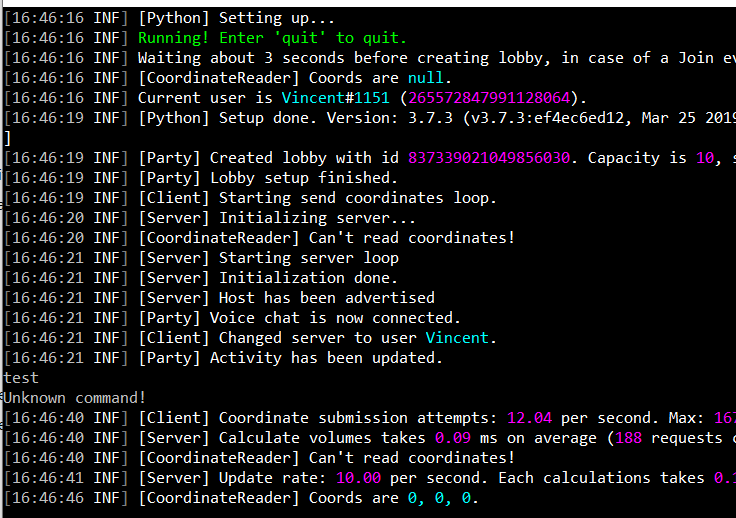
\includegraphics[trim={0px 90px 0px 5px},clip,width=\linewidth,height=0.4\textheight,keepaspectratio]{assets/consoleOutput.png}
            \end{column}
        \end{columns}
    \end{frame}

    \addtorecentlist{\LaTeX}

    \begin{frame}
        \frametitle{\LaTeX: Tekst vs Visueel}
        
        \begin{itemize}
        	\item Veel informatie
        	\begin{itemize}
        		\item Formules
        		\item Diagrammen
        		\item {\setul{1pt}{1pt}\setulcolor{green}\ul{Fanciness}} {\setul{0pt}{1pt}\st{Fancyness}}
        	\end{itemize}
        
        	\item Minimalistische informatie
        	\begin{itemize}
        		\item Herhalende elementen
        		\item Consistentie
        	\end{itemize}
        	
        	\item Simpele informatie
        	\begin{itemize}
        		\item Veel packages voor allerlei aanpassingen, allerlei \adjustbox{scale={1}{-1},valign=b}{\setul{1pt}{1pt}\setulcolor{blue}\ul{Fanciness}}.
        	\end{itemize}
        	
            %\item \textfrak{\so{S{ch}u{tz}vorri{ch}tung}}
        \end{itemize}
    
    	\pause
    	Maar: \"F\textsl{\H{a}nc}\^{\i}\~ne\c{s}s is vaak DIY, en kost al snel veel moeite!
    \end{frame}

	\begin{saveblock}{repeatel}
		\begin{highlightblock}[linewidth=0.5\textwidth,gobble=12]
			\begin{lemma}
				Lorem ipsum dolor sit
				... eget dolor.
				
				\begin{proof}
					Aenean massa. Cum
					... quis enim.
				\end{proof}
			\end{lemma}
		\end{highlightblock}
	\end{saveblock}

	\begin{frame}
		\frametitle{\LaTeX: Tekst vs Visueel}
		\begin{columns}
			\begin{column}{0.5\textwidth}
				\useblock{repeatel}
			\end{column}
			\begin{column}{0.5\textwidth}
				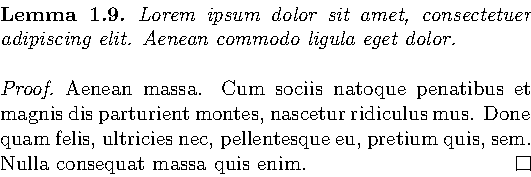
\includegraphics[width=\linewidth,height=0.8\textheight,keepaspectratio]{assets/latexRepeatEl.pdf}
			\end{column}
		\end{columns}
	\end{frame}
    
    \begin{frame}
        \frametitle{Word: Tekst vs Visueel}
        
        \begin{itemize}
            \item Gaat kopiëren van een tabel wel goed? Blijft de opmaak dan goed behouden?
            \item Waar komt die witruimte opeens vandaan?
            \item Waarom wil Word de volgende regel opeens in bold?
        \end{itemize}
    
    \end{frame}
    
    %\begin{frame}
    %	\LaTeX{} $ \simeq $ Word
    %\end{frame}
    %
    %\begin{frame}
    %	Websites niet via Word
    %\end{frame}
    %
    %\begin{frame}
    %	Apps niet via Word
    %\end{frame}
    %
    %\begin{frame}
    %	Wikipedia niet via Word
    %\end{frame}
    
    %\begin{frame}[<+->]
    %	Problemen met Word:
    %	\begin{enumerate}
    %		\item Informatie $\leftrightarrow$ Visueel
    %			\begin{itemize}
    %				\item Formules
    %				\item Geavanceerde diagramplaatsing
    %				\item Buiten documenten: schermgrootte, website links, \textellipsis
    %			\end{itemize}
    %		\item Betekenis $ \leftrightarrow $ Visueel
    %			\begin{itemize}
    %				\item Vaste elementen (bv. `Voorbeeld' of `Opmerking' boxen)
    %				\item Geen verspringende opmaken of spookwitruimte
    %				\item Door code: gebruik een package voor een bijzondere wens, of schrijf code zelf.
    %			\end{itemize}
    %	\end{enumerate}
    %\end{frame}
    
    
    % \begin{frame}
    % 	\frametitle{Overleaf}
    
    % 	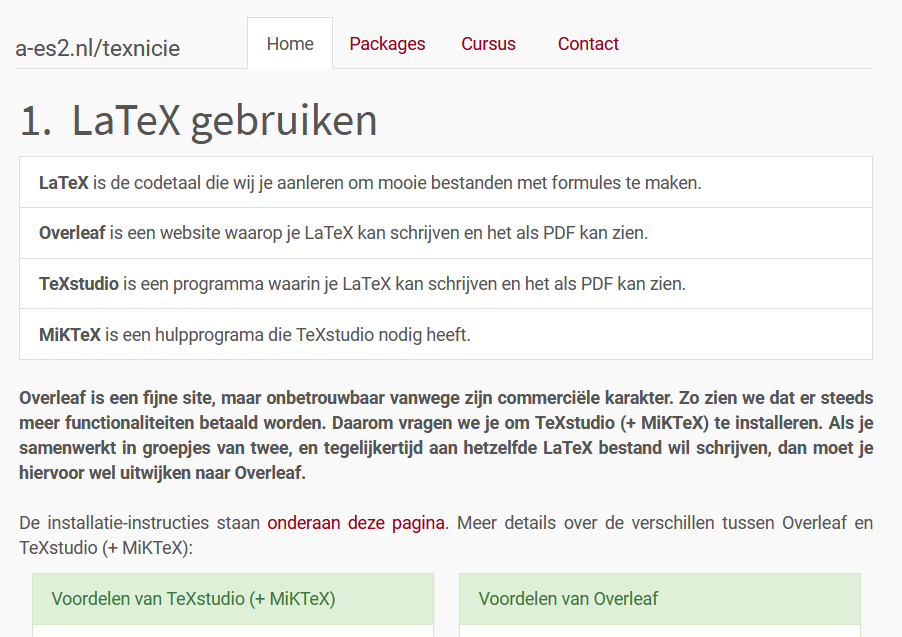
\includegraphics[height=0.85\textheight]{texnicieWebsiteOverleafTeXstudio.png}
    % \end{frame}

    \addtorecentlist{Overleaf}
    
    \begin{frame}
        \frametitle{Overleaf}
    
        %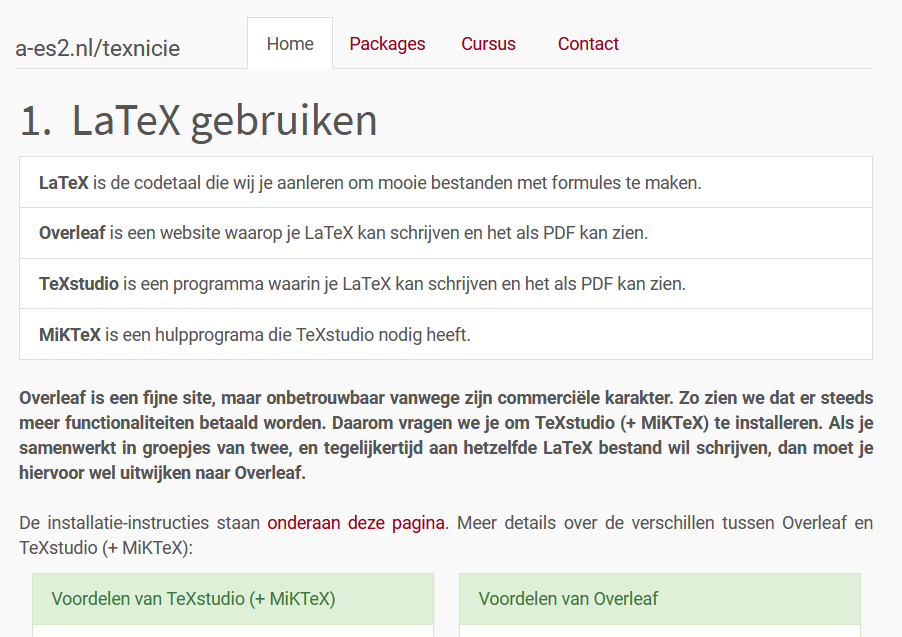
\includegraphics[trim=10px 120px 50px 30px,clip,width=0.95\textwidth]{texnicieWebsiteOverleafTeXstudio.png}
        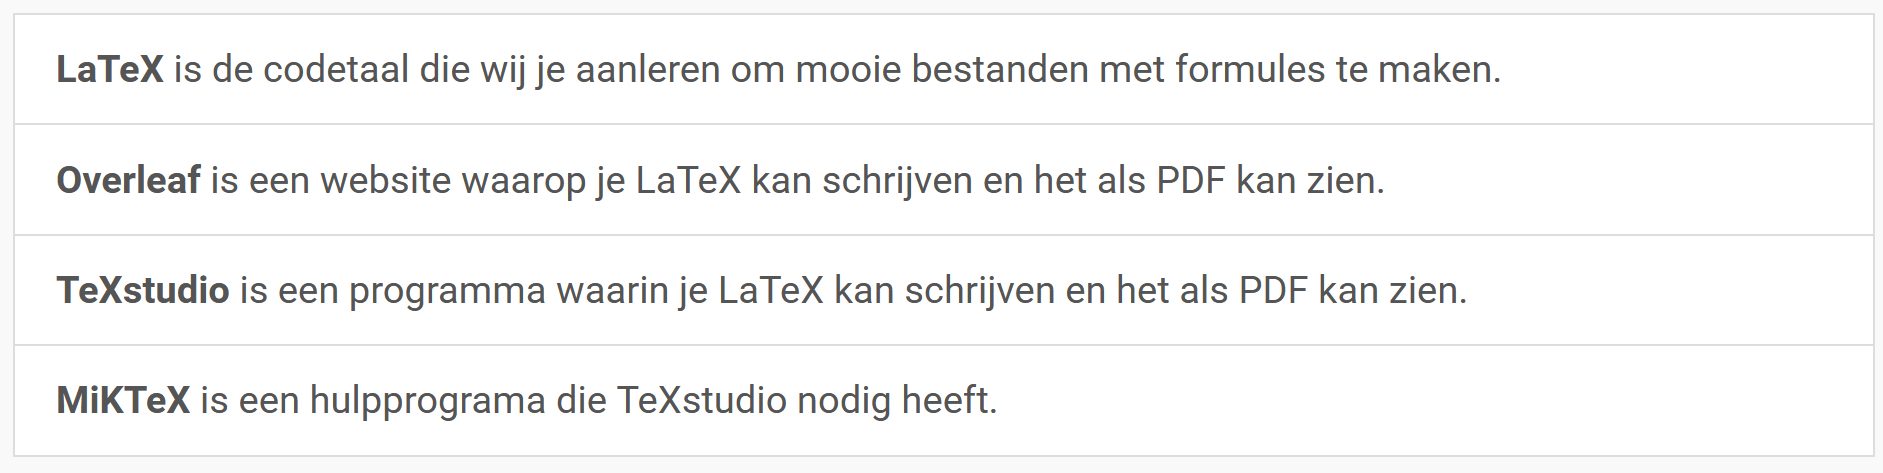
\includegraphics[width=\textwidth]{assets/overleafDisambiguation.png}
    
        \begin{columns}
            \begin{column}{0.3\textwidth}
                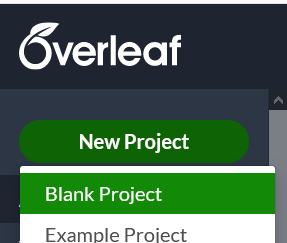
\includegraphics[width=\linewidth]{assets/overleafCreateBlankProject.png}
            \end{column}
            \begin{column}{0.7\textwidth}
                Op het einde nog woordje hierover.
                
                Voor nu: Overleaf.
                
                \medskip
                Nu al niet-commerci\"ele variant installeren? \url{a-es2.nl/texnicie}
            \end{column}
        \end{columns}
    \end{frame}
    
    \begin{saveblock}{baseDocument}
        \begin{highlightblock}[linewidth=0.5\textwidth,gobble=12]
            \documentclass{article}
            \usepackage[utf8]{inputenc}
    
            \title{My document}
            \author{Vincent Kuhlmann}
            \date{1 May 2021}
    
            \begin{document}
            \maketitle
            \section{Introduction}
    
            Hallo iedereen!
            \end{document}
        \end{highlightblock}
    \end{saveblock}

    \addtorecentlist{Simpel document}
    
    \begin{frame}
        \frametitle{Simpel document}
    
        \begin{columns}
            \begin{column}{0.5\textwidth}
                \useblock{baseDocument}
            \end{column}
            \begin{column}{0.5\textwidth}
                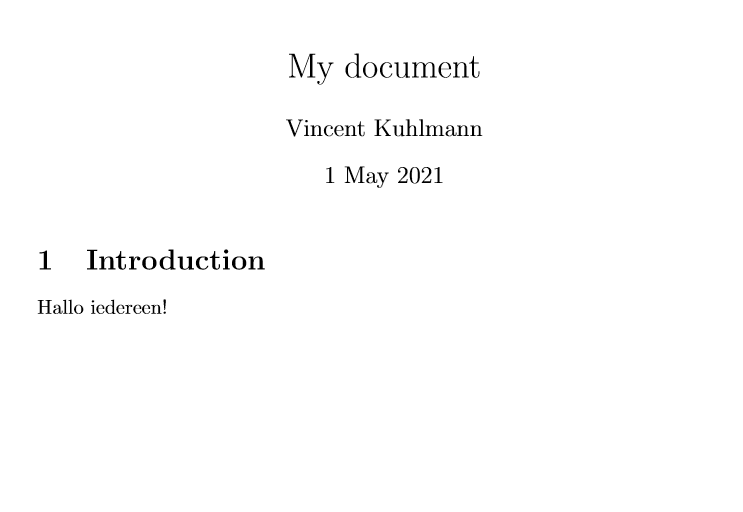
\includegraphics[width=\linewidth]{assets/basicDocumentOutput.png}
            \end{column}
        \end{columns}
    \end{frame}
\end{document}
